% --- chapter
\newcommand{\chapter}[2][]{
	\newcommand{\chapname}{#2}
	\begin{flushleft}
		\begin{minipage}[t]{\linewidth}
			
\includegraphics[height=1cm]{hdht-logo.png}
			\hspace{0pt}	
			\sffamily\bfseries\large Bài  25. Giao thoa ánh sáng
			\begin{flushleft}
				\huge\bfseries #1
			\end{flushleft}
		\end{minipage}
	\end{flushleft}
	\vspace{1cm}
	\normalfont\normalsize
}
%-----------------------------------------------------
\chapter[Giao thoa nhiều ánh sáng đơn sắc]{Giao thoa nhiều ánh sáng đơn sắc}

\begin{dang}{Số vạch sáng trùng nhau khi giao thoa hai ánh sáng đơn sắc.}
\ppgiai{
Giả sử trên đoạn AB trên màn đếm được $\text{N}_{\text{vs}}$ vạch sáng.	

Mỗi ánh sáng đơn sắc cho một hệ vân giao thoa riêng. Mỗi vân sáng là một vạch sáng, nhưng nếu vân sáng hệ này trùng vân sáng hệ kia thì ở vị trí đó chỉ có một vạch sáng (vân sáng trùng). 
\begin{description}
\item [Bước 1] Gọi $\text{N}_1$, $\text{N}_2$ lần lượt là tổng số vân sáng trên AB khi giao thoa lần lượt với $\lambda_1$, $ \lambda_2$.
\item [Bước 2] Số vân trùng trên AB là $N = \text{N}_1 + \text{N}_2 -\text{N}_{\text{vs}}$.
\item [Bước 3] Để tìm $\text{N}_1$, $\text{N}_2$ ta chú ý, với mỗi ánh sáng $\lambda_j$:
\begin{itemize}
	\item Tại A và B là hai vân sáng $N_j=\dfrac{AB}{i_j}+1.$
	\item Tại A và B là hai vân tối $N_j=\dfrac{AB}{i_j}.$
	\item Tại A là vân sáng và tại B là vân tối $N_j=\dfrac{AB}{i_j}+ \text{0,5}$.
	\item Tại A là vân sáng và tại B chưa biết $N = \left[\dfrac{AB}{i}\right]+1$.
	\item Tại A là vân tối và tại B chưa biết $ N=\left[\dfrac{AB- \text{0,5}i}{i}\right]+1.$
\end{itemize}
trong đó kí hiệu [..] nghĩa là lấy phần nguyên.
\end{description}
}

\viduii{3}
	{
		Trong thí nghiệm giao thoa Iâng, thực hiện đồng thời với hai ánh sáng đơn sắc thì khoảng vân lần lượt 0,64 mm và 0,54 mm. Xét tại hai điểm A, B trên màn cách nhau một khoảng 34,56 mm là hai vị trí mà cả hai hệ vân đều cho vân sáng tại đó. Trên khoảng đó quan sát được 117 vạch sáng. Hỏi trên AB có mấy vạch sáng là kết quả trùng nhau của hai hệ vân.
		\begin{mcq}(4)
			\item  3.			
			\item  4.				
			\item  5.			
			\item  1.
		\end{mcq}
	}
	{
		\begin{center}
			\textbf{Hướng dẫn giải}
		\end{center}
\begin{itemize}
\item Số vân trùng 
\begin{equation*} 
N = N_1+N_2-N_{\text{vs}}=\left(\dfrac{AB}{i_1}+1\right) +\left(\dfrac{AB}{i_2}+1\right) - N_{\text{vs}}.
\end{equation*}
\item Thay số vào $N=3.$
\end{itemize}

	\begin{center}
		\textbf{Câu hỏi tương tự}
	\end{center}

Trong thí nghiệm giao thoa ánh sáng, thực hiện đồng thời hai bức xạ đơn sắc với khoảng vân trên màn lần lượt là $ \SI{0,48}{mm} $ và $ \SI{0,54}{mm} $. Tại hai điểm $ A $ và $ B $ trên màn cách nhau một khoảng $ \SI{51,84}{mm} $ là hai vị trí mà cả hai vân đều cho vân sáng tại đó. Số vạch sáng là kết quả trùng nhau của hai hệ vân trên đoạn $ AB $ là
\begin{mcq}(4)
			\item 11.			
			\item 12.				
			\item 13.			
			\item 14.
		\end{mcq}

\textbf{Đáp án:} C.
}

\viduii{3}
	{
Một nguồn sáng điểm nằm cách đều hai khe lâng và phát ra đồng thời hai bức xạ đơn sắc có bước sóng 0,6 $\mu$m và bước sóng $\lambda$  chưa biết. Khoảng cách hai khe 1 mm, khoảng cách từ hai khe đến màn 2 m. Trong một khoảng rộng L = 24 mm trên màn, đếm được 33 vạch sáng, trong đó có 5 vạch là kết quả trùng nhau của hai hệ vân. Tính bước sóng $\lambda$, biết hai trong 5 vạch trùng nhau nằm ngoài cùng của khoảng L.
\begin{mcq}(4)
\item 0,45 $\mu$m.		
\item 0,55 $\mu$m.			
\item 0,65 $\mu$m.		
\item 0,75 $\mu$m.
\end{mcq}
}
	{
		\begin{center}
			\textbf{Hướng dẫn giải}
		\end{center}
\begin{itemize}
	\item Khoảng vân ánh sáng có bước sóng $\lambda_1$
	
	\begin{equation*}
		i_1=\dfrac{\lambda_1 D}{a}= \SI{1,2}{mm}.
	\end{equation*}

	\item Công thức tính số vân trùng
	
	\begin{equation*}
		N= \left(\dfrac{AB}{i_1}+1\right) +\left(\dfrac{AB}{i_2}+1\right) - N_{\text{vs}}.
	\end{equation*}

	\item Suy ra $i_2= \SI{1,5}{mm}$. 
	\item Từ $i_2$ tìm được $\lambda_2 =\dfrac{ai_2}{D}=\text{0,75}\ \mu \text{m}$.
\end{itemize}

		\begin{center}
			\textbf{Câu hỏi tương tự}
		\end{center}

Một nguồn sáng điểm nằm cách đều hai khe Y-âng và phát ra đồng thời hai bức xạ đơn sắc có bước sóng $ \lambda_{1} = \SI{0,6}{\mu m} $ và $ \lambda_{2} $ chưa biết. Khoảng cách hai khe là $ a = \SI{0,2}{mm} $, khoảng cách từ hai khe đến màn là $ D = \SI{1}{m} $. Trên một khoảng rộng $ L = \SI{2,4}{cm} $ trên màn, đếm được $ 17 $ vạch sáng, trong đó có $ 3 $ vạch là kết quả trùng nhau của hai hệ vân và hai trong ba vạch trùng nhau nằm ngoài cùng của khoảng $ L $. Giá trị của $ \lambda_{2} $ là
\begin{mcq}(2)
	\item $ \lambda_{2} = \SI{0,8}{\mu m} $.
	\item $ \lambda_{2} = \SI{0,24}{\mu m} $.
	\item $ \lambda_{2} = \SI{0,12}{\mu m} $.
	\item $ \lambda_{2} = \SI{0,48}{\mu m} $.
\end{mcq}
\textbf{Đáp án:} D.
}
\end{dang}

\begin{dang}{Số vạch sáng nằm giữa vân sáng bậc $k_1$ của $\lambda_1$ và vân sáng bậc $k_2$ của $\lambda_2$.}

\ppgiai{
	\begin{description}
	\item[Cách giải 1:] (áp dụng cho $k_1$ và $k_2$ không quá lớn, có thể vẽ hình để liệt kê)
	\begin{description}
		\item [Bước 1] Vân sáng trùng nhau: 
		\begin{equation*}
		x=k_1\dfrac{\lambda_1 D}{a}=k_2 \dfrac{\lambda_2 D}{a} \Rightarrow \dfrac{k_1}{k_2}=\dfrac{\lambda_1}{\lambda_2} = \text{phân số tối giản}= \dfrac{b}{c}
		\end{equation*}
		\item [Bước 2] Vẽ các vân trùng cho đến bậc $k_1$ của hệ 1 và bậc $k_2$ của hệ 2.
		\item [Bước 3] Từ hình vẽ xác định được số vạch sáng.
	\end{description}

	\item[Cách giải 2:] (áp dụng nếu $k_1$ hoặc $k_2$ quá lớn để vẽ)
	\begin{description}
		\item [Bước 1] Vân sáng trùng nhau: 
		\begin{equation*}
		x=k_1\dfrac{\lambda_1 D}{a}=k_2 \dfrac{\lambda_2 D}{a} \Rightarrow \dfrac{k_1}{k_2}=\dfrac{\lambda_1}{\lambda_2} = \text{phân số tối giản}= \dfrac{b}{c}
		\end{equation*}
		\item [Bước 2] Tìm số vân trùng nhau giữa hai vị trí đề bài cho.
		\item [Bước 3] Áp dụng công thức tính số vân sáng giữa hai điểm (xem mục 1), tìm số vân sáng của mỗi ánh sáng giữa hai vị trí đề bài cho.
		\item [Bước 4] Tính số vân sáng bằng công thức
		$$N=N_1+N_2-N_\textrm{trùng}.$$
	\end{description}
	
\end{description}
}

\viduii{3}
	{
Trong thí nghiệm về giao thoa ánh sáng, chiếu đồng thời vào hai khe hai bức xạ có bước sóng $\lambda_1 = \text{0,42}\ \mu \text{m}$ và $\lambda_1 = \text{0,525}\ \mu \text{m}$. Hệ thống vân giao thoa được thu hên màn, tại điểm M trên màn là vân sáng bậc 4 của bức xạ $\lambda_1$ , và điểm N là vân sáng bậc 11 của bức xạ $\lambda_2$. Biết M và N nằm cùng về một phía so với vân sáng trung tâm. Trừ hai vạch sáng tại hai điểm M, N thì trong đoạn MN có
\begin{mcq}(2)
\item 15 vạch sáng. 
\item 13 vạch sáng. 		
\item 16 vạch sáng.  		 
\item 14 vạch sáng.
\end{mcq}
}
{\begin{center}
	\textbf{Hướng dẫn giải}
\end{center}
\textbf{Cách giải 1:}
\begin{itemize}
	\item Lập tỉ số: 
	c
	\item Vẽ vị trí trùng đầu tiên là $k_1 = 0, k_2 = 0$, tiếp đến $k_1 = 5, k_2 = 4$, rồi $k_1 = 10, k_2 = 8$ và $k_1 = 15, k_2 = 12$.
	\item Xác định điểm M là vân sáng bậc 4 của hệ 1 và điểm N là vân sáng bậc 11 của hệ 2.
	\item Trong khoảng MN (trừ M và N) có: 
	
\begin{center}
	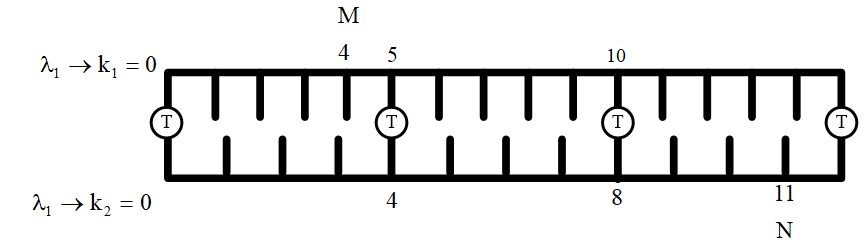
\includegraphics[scale=0.7]{../figs/VN12-PH-33-A-017-2-1.JPG}
\end{center}	
	
	+ 2 vạch trùng nhau.
	
	+ $13-4=9$ vân sáng hệ 1.
	
	+ $11-4=7$ vân sáng hệ 2.
	\item Tổng số vạch sáng trên khoảng MN: $9+7-2=14$.   
	
\end{itemize}

\textbf{Cách 2:}

\begin{itemize}
	\item Lập tỉ số: 
	\begin{equation*}
		\dfrac{i_1}{i_2}=\dfrac{\lambda_1}{\lambda_2}=\dfrac{4}{5} \Rightarrow i_1=4i, i_2=5i \Rightarrow i'=4\cdot 5i=20i.
	\end{equation*}
	\item Tọa độ của M và N: $x_{\text{M}}=4i_1=16i$ và $x_{\text{N}}=11i_2=55i$.
	\item Số vân sáng của hệ 1, hệ 2 và số vân trùng trong khoảng MN (trừ M và N, điều kiện ($16i < x < 55i$) được xác định: 
	\begin{equation*}
	16i < k_1i_1  < 55i \Rightarrow 16i<k_1\cdot 4i<55i \Rightarrow 4<k_1< \text{13,75} \Rightarrow k_1=5;...;13\ \text {có 9 giá trị}.
	\end{equation*}

	\begin{equation*}
	16i < k_2i_2  < 55i \Rightarrow 16i<k_2\cdot 5i<55i \Rightarrow \text{3,2}<k_2< 11 \Rightarrow k_2=4;...;10\ \text {có 7 giá trị}.
	\end{equation*}

	\begin{equation*}
	16i < k'i'  < 55i \Rightarrow 16i<k'\cdot 20i<55i \Rightarrow \text{0,8}<k'< \text{2,75} \Rightarrow k'=1; 2\ \text {có 2 giá trị}.
	\end{equation*}

	\item Tổng số vạch sáng trên khoảng MN: $9+7-2=14$.  
\end{itemize}

		\begin{center}
			\textbf{Câu hỏi tương tự}
		\end{center}
Trong thí nghiệm về giao thoa ánh sáng, chiếu đồng thời vào hai khe hai bức xạ có bước sóng $ \lambda_{1} = \SI{0,42}{\mu m} $ và $ \lambda_{2} = \SI{0,525}{\mu m} $. Hệ thống vân giao thoa thu được trên màn, tại điểm $ M $ trên màn là vân sáng bậc $ 4 $ của bức xạ $ \lambda_{2} $, và điểm $ N $ là vân sáng bậc $ 10 $ của bức xạ $ \lambda_{1} $. Biết $ M $ và $ N $ nằm cùng về một phía so với vân sáng trung tâm. Trừ hai vạch sáng tại $ M $ và $ N $ thì trong đoạn $ MN $ có
\begin{mcq}(2)
	\item $ 10 $ vân sáng.
	\item $ 9 $ vân sáng.
	\item $ 8 $ vân sáng.
	\item $ 7 $ vân sáng.
\end{mcq}
\textbf{Đáp án:} D.
}

\viduii{3}
{
Trong thí nghiệm về giao thoa ánh sáng, chiếu đồng thời vào hai khe hai bức xạ có bước sóng $\lambda_1 = \text{0,6}\ \mu \text{m}$ và $\lambda_2 = \text{0,4}\ \mu \text{m}$. Hệ thống vân giao thoa được thu trên màn, tại điểm M trên màn là vân tối thứ 4 của bức xạ $\lambda_1$, và điểm N là vân sáng bậc 17 của bức xạ $\lambda_2$. Biết M và N nằm cùng về một phía so với vân sáng trung tâm. Trừ hai điểm M, N thì trong khoảng MN có
\begin{mcq}(2)
\item 16 vạch sáng. 	
\item 14 vạch sáng.   	
\item 20 vạch sáng. 	   
\item 15 vạch sáng.
\end{mcq}
}
{\begin{center}
	\textbf{Hướng dẫn giải}
\end{center}

\begin{itemize}
	\item Lập tỉ số: 
	\begin{equation*}
		\dfrac{i_1}{i_2}=\dfrac{\lambda_1}{\lambda_2}=\dfrac{3}{2} \Rightarrow i_1=3i, i_2=2i \Rightarrow i'=3\cdot 2i=6i.
	\end{equation*}
	\item Tọa độ của M và N: $x_{\text{M}}=\text{3,5}i_1=\text{10,5}i$ và $x_{\text{N}}=17i_2=34i$.
	\item Số vân sáng của hệ 1, hệ 2 và số vân trùng trong khoảng MN (trừ M và N, điều kiện ($\text{10,5}i < x < 34i$) được xác định: 
	\begin{equation*}
		\text{10,5}i < k_1i_1  < 34i \Rightarrow \text{10,5}i<k_1\cdot 3i<34i \Rightarrow \text{3,5}<k_1< \text{11,3} \Rightarrow k_1=4;...;11\ \text {có 8 giá trị}.
	\end{equation*}
	
	\begin{equation*}
		\text{10,5}i < k_2i_2  < 34i \Rightarrow \text{10,5}i<k_2\cdot 2i<34i \Rightarrow \text{5,25}<k_2< 17 \Rightarrow k_2=6;...;16\ \text {có 11 giá trị}.
	\end{equation*}
	
	\begin{equation*}
		\text{10,5}i < k'i'  < 34i \Rightarrow \text{10,5}i<k'\cdot 6i<34i \Rightarrow \text{1,75}<k'< \text{5,6} \Rightarrow k'=2;...5\ \text {có 2 giá trị}.
	\end{equation*}
	
	\item Tổng số vạch sáng trên khoảng MN: $8+11-4=15$.  
\end{itemize}

		\begin{center}
			\textbf{Câu hỏi tương tự}
		\end{center}
		
Trong thí nghiệm về giao thoa ánh sáng, chiếu đồng thời vào hai khe bức xạ có bước sóng $ \lambda_{1} $ và $ \lambda_{2} = 0,75 \lambda_{1} $. Hệ thống vân giao thoa được thu trên màn, tại điểm $ M $ trên màn là vân sáng bậc 1 của bức xạ $ \lambda_{1} $, và điểm $ N $ là vân sáng bậc 7 của bức xạ $ \lambda_{2} $. Biết $ M $ và $ N $ nằm cùng một phía so với vân sáng trung tâm. Trừ hai vạch sáng tại điểm $ M, N $ thì trong đoạn $ MN $ có
\begin{mcq}(2)
	\item $ 6 $ vạch sáng.
	\item $ 4 $ vạch sáng.
	\item $ 7 $ vạch sáng.
	\item $ 8 $ vạch sáng.
\end{mcq}

\textbf{Đáp án:} D.
}
\luuy{\begin{itemize}
		\item  Bài toán liên quan đến bậc vân không quá lớn nên giải theo cách 1.
		\item  Bài toán liên quan đến bậc vân lớn hoặc liên quan đến vân tối hoặc liên quan đến tọa độ nên giải theo cách 2.
	\end{itemize}
}
\end{dang}

\begin{dang}{Xác định bước sóng khi biết các vân\\ trùng nhau.}
\ppgiai{

\begin{description}
	\item [Bước 1] Xác định các yếu tố đề bài cho: 
	\begin{itemize}
		\item Vân sáng trùng vân sáng
	\begin{equation*}
		x=k_1\dfrac{\lambda_1 D}{a}=k_2\dfrac{\lambda_2 D}{a}.
	\end{equation*}
		\item Vân sáng trùng vân tối 
		\begin{equation*}
			x=k_1\dfrac{\lambda_1 D}{a}=(m_2 + \text{0,5})\dfrac{\lambda_2 D}{a}.
		\end{equation*}
		\item Vân tối trùng vân tối 
		\begin{equation*}
		x=(m_1 + \text{0,5})\dfrac{\lambda_1 D}{a}=(m_2 + \text{0,5})\dfrac{\lambda_2 D}{a}.
		\end{equation*}
		
	\end{itemize}
	
	\item [Bước 2] Biểu diễn $\lambda$ theo $k$ hoặc $m$ rồi thay vào điều kiện giới hạn $\text{0,38}\ \mu \text{m} \leq  \lambda \leq  \text{0,76}\ \mu \text{m}$, giải tìm $k$ hoặc $m$, từ đó suy ra $lambda$. 
\end{description}
}

\viduii{3}
{	
Trong thí nghiệm Y-âng, của hai bước sóng $\lambda_1 = \text{0,72}\ \mu \text{m}$ và $\lambda_2$ , người ta thấy vân sáng bậc 3 của bức xạ $\lambda_2$ trùng với vân sáng bậc 2 của bức xạ $\lambda_1$. Tìm $\lambda_1$. 
\begin{mcq}(2)
\item $\lambda_2 = \text{0,54}\ \mu \text{m}$.		
\item $\lambda_2 = \text{0,43}\ \mu \text{m}$.		
\item $\lambda_2 = \text{0,48}\ \mu \text{m}$. 
\item $\lambda_2 = \text{0,45}\ \mu \text{m}$.
\end{mcq}
}
{\begin{center}
	\textbf{Hướng dẫn giải}
 \end{center}

\begin{itemize}
	\item Vân sáng trùng vân sáng
	\begin{equation*}
		x=2\dfrac{\lambda_1 D}{a}=3\dfrac{\lambda_2 D}{a}.
	\end{equation*}
	\item Suy ra $\lambda_2=2\dfrac{\lambda_1}{3} = \text{0,48}\ \mu \text{m}$
\end{itemize}

\begin{center}
	\textbf{Câu hỏi tương tự}
	\end{center}
Trong thí nghiệm Y-âng về giao thoa ánh sáng hai khe cách nhau $ \SI{1}{mm} $, khoảng cách từ hai khe đến màn là $ \SI{2}{m} $. Nếu chiếu đồng thời hai bức xạ đơn sắc có bước sóng $ \lambda_{1} = \SI{0,602}{\mu m} $  và $ \lambda_{2} $ thì thấy vân sáng bậc 3 của bức xạ $ \lambda_{2} $ trùng với vân sáng bậc $ 2 $ của bức xạ $ \lambda_{1} $. Giá trị của $ \lambda_{2} $ là
\begin{mcq}(4)
	\item $ \SI{0,402}{\mu m} $.
	\item $ \SI{0,502}{\mu m} $.
	\item $ \SI{0,603}{\mu m} $.
	\item $ \SI{0,704}{\mu m} $.
\end{mcq}
\textbf{Đáp án:} A.
}
 
\viduii{3}
{Trong thí nghiệm giao thoa lâng, thực hiện đồng thời với hai ánh sáng đơn sắc  $\lambda_1$ và $\lambda_2 = \SI{0,5}{\mu m} $. Xác định $\lambda_1$ để vân sáng bậc 3 của $\lambda_2$ trùng với một vân tối của $\lambda_1$. Biết $\text{0,58}\ \mu \text{m} \leq \lambda_2 \leq \text{0,76}\ \mu \text{m}$.
\begin{mcq}(4)
\item  0,6 $\mu$m.			
\item  0,5 $\mu$m.			
\item  0,45 $\mu$m.			
\item  0,65 $\mu$m.
\end{mcq}
}
{\begin{center}
	\textbf{Hướng dẫn giải}
\end{center}
\textbf{Cách giải 1}

\begin{itemize}
	\item Vân sáng trùng vân tối 
	\begin{equation*}
		x=3\dfrac{\lambda_1 D}{a}=(m_2 - \text{0,5})\dfrac{\lambda_2 D}{a}.
	\end{equation*}
	\item Suy ra 
	\begin{equation*}
	\lambda_2= \dfrac{3\cdot \text{0,5}}{m_2-\text{0,5}}\ \mu \text{m}. 
	\end{equation*}
	\item Thay $\lambda_2$ vào được 
	\begin{equation*}
		 \text{0,58}\ \mu \text{m} \leq \dfrac{3\cdot \text{0,5}}{m+\text{0,5}} \leq \text{0,76}\ \mu \text{m},\\
		 \Leftrightarrow \text{1,47} \leq m \leq \text{2,08}, \\
		 \Rightarrow m =2.
	\end{equation*}

	\item Suy ra $\lambda = \text{0,6}\ \mu \text{m}$
	
\textbf{Cách giải 2}

Sử dụng máy tính bỏ túi 

\begin{description}
	\item [Bước 1] Sau khi đã biến đổi $\lambda_2$ theo $m$, chọn MODE 7
	\item [Bước 2] Màng hình hiển thị f(X) =, nhập biểu thức $\dfrac{\text{1,5}}{X+\text{0,5}}.$
	\item [Bước 3] Start? 1  nhấn dấu =.
	\item [Bước 4] End? 10 nhấn dấu =.
	\item [Bước 5]Step? 1 nhấn dấu =.
	\item [Bước 6] Hiển thị bảng gồm 3 cột số thứ tự, X và F(X), chọn giá trị tương ứng ứng với X là $m$ và F(X) là $\lambda_2$ thỏa mãn với biểu thức $\text{0,58}\ \mu \text{m} \leq \lambda_2 \leq \text{0,76}\ \mu \text{m}$.
\end{description}
	
\end{itemize}

\begin{center}
	\textbf{Câu hỏi tương tự}
	\end{center}
	
Trong thí nghiệm giao thoa Y-âng, thực hiện đồng thời hai ánh sáng đơn sắc $ \lambda_{1} $ và $ \lambda_{2} = \SI{0,4}{\mu m} $. Xác định $ \lambda_{1} $ để vân sáng bậc 2 của $ \lambda_{2} $ trùng với vân tối của $ \lambda_{1} $. Biết $ \SI{0,38}{\mu m} \leq \lambda_{1} \leq \SI{0,76}{\mu m} $.
\begin{mcq}(4)
	\item $ \SI{0,60}{\mu m} $.
	\item $ \SI{0,53}{\mu m} $.
	\item $ \SI{0,47}{\mu m} $.
	\item $ \SI{0,65}{\mu m} $.
\end{mcq}

\textbf{Đáp án:} B.
}

\end{dang}

\begin{dang}{Vạch sáng cùng màu với vạch sáng\\ trung tâm.}

\ppgiai{
Khi giao thoa Y-âng thực hiện đồng thời với n ánh sáng đơn sắc thì mỗi ánh sáng cho một hệ thống vân giao thoa riêng.

Tại trung tâm là nơi trùng nhau của tất cả các vân sáng bậc 0 và tại đây sẽ có một màu nhất định (chẳng hạn đỏ trùng với xanh lục sẽ được màu vàng).

Nếu tại điểm M trên màn có vạch sáng cùng màu với vạch sáng trung tâm thì tại đây cũng phải trùng đầy đủ các vân sáng của các hệ giống như vân trung tâm: $$x=k_1i_1=k_2i_2=...=k_ni_n.$$

\subsubsection{Trường hợp 2 bức xạ}

Đây chính là bài toán liên quan đến hai vân sáng của hai hệ trùng nhau mà ta đã khảo sát. Tuy nhiên, sẽ có nhiều vấn đề mới sẽ được khai thác thêm.

\begin{description}
	\item [Bước 1] Lập tỉ số tối giản	
	\begin{equation*}
		\dfrac{i_2}{i_1}=\dfrac{b}{c}. 
	\end{equation*}
	\item [Bước 2] Tìm khoảng vân trùng 
	\begin{equation*}
		i'=bi_1=ci_2.
	\end{equation*}	
	\item [Bước 3] Tìm vị trí vân trùng $$x = n i',$$
	
	\item [Bước 4] Dựa vào điều kiện $x_{\text{M}} \leq ni' \leq x_{\text{N}}$ và số vân trùng $N=2\left[\dfrac{\text{0,5} L}{i'}\right] +1$ để xác định các đại lượng cần tìm.
\end{description}	
\subsubsection{Trường hợp 3 bức xạ}

Khi giao thoa Y-âng thực hiện đồng thời với 3 ánh sáng đơn sắc thì mỗi ánh sáng cho một hệ thống vân giao thoa riêng.

Tại trung tâm là nơi trùng nhau của 3 vân sáng bậc 0 của ba hệ vân và tại đây sẽ có một màu nhất định (chẳng hạn đỏ, lục lam chồng lên nhau sẽ được màu trắng).

Nếu tại điểm M trên màn có vạch sáng cùng màu với vạch sáng trung tâm thì tại đây ba vân sáng của 3 hệ trùng nhau $x=k_1i_1=k_2i_2=k_3i_3.$


\begin{description}
	\item [Bước 1] Lập các tỉ số
	\begin{equation*}
	\dfrac{k_1}{k_2}=\dfrac{i_2}{i_1}=\dfrac{b_1}{c_1}=\dfrac{b}{c}.
	\end{equation*}
	\begin{equation*}
		\dfrac{k_3}{k_2}=\dfrac{i_2}{i_3}=\dfrac{b_2}{c_2}=\dfrac{d}{c}.
	\end{equation*}
	\item [Bước 2] Tìm khoảng vân trùng 
	\begin{equation*}
		i'=bi_1=ci_2 =di_3.
	\end{equation*}	
	\item [Bước 3] Tìm vị trí vân trùng $x = n i'$.
	\item [Bước 4]Dựa vào điều kiện $x_{\text{M}} \leq ni' \leq x_{\text{N}}$ và số vân trùng $N=2\left[\dfrac{\text{0,5} L}{i'}\right] +1$ để xác định các đại lượng cần tìm.
\end{description}
}

\viduii{2}
{Trong thí nghiệm giao thoa Y-âng, thực hiện đồng thời với hai ánh sáng đơn sắc khoảng vân giao thoa lần lượt là 1 mm và 1,5 mm. Xác định vị trí các vạch sáng cùng màu với vạch sáng trung tâm (n là số nguyên)
\begin{mcq}(2)
\item $x =$ 2,5n mm. 	
\item $x =$ 4n mm.   	  
\item $x =$ 4,5n mm.          
\item $x =$ 3n mm. 
\end{mcq}
}
{\begin{center}
	\textbf{Hướng dẫn giải}
\end{center}

\begin{itemize}
	\item Lập tỉ số
	\begin{equation*}
		\dfrac{i_2}{i_1}=\dfrac{3}{2}.
	\end{equation*}
	\item Khoảng vân trùng
	\begin{equation*}
		i'=3i_1=2i_2= 3\ \text{mm}.
	\end{equation*}
	\item Vị trí vân sáng cùng màu với vân sáng trung tâm
	\begin{equation*}
	x=ni'=3n\ \text{mm}
	\end{equation*}
\end{itemize}

\begin{center}
	\textbf{Câu hỏi tương tự}
\end{center}

Trong thí nghiệm giao thoa Y-âng, thực hiện đồng thời với hai ánh sáng đơn sắc khoảng vân giao thoa lần lượt là 1,5 mm và 2,0 mm. Xác định vị trí các vạch sáng cùng màu với vạch sáng trung tâm (n là số nguyên)
\begin{mcq}(2)
\item $x =$ 6n mm. 	
\item $x =$ 5n mm.   	  
\item $x =$ 4n mm.          
\item $x =$ 3n mm. 
\end{mcq}

\textbf{Đáp án:} A.
}
\viduii{2}
{Thí nghiệm giao thoa Yâng thực hiện đồng thời hai ánh sáng đơn sắc thì khoảng vân giao thoa lần lượt là 1,125mm và 0,75 mm. Bề rộng trường giao thoa trên màn là 10 mm. Số vạch sáng cùng màu với vạch sáng trung tâm (kể cả vạch sáng trung tâm) là
\begin{mcq}(4)
\item 3.			
\item 4.				
\item 5.				
\item 6.
\end{mcq}
}
{\begin{center}
	\textbf{Hướng dẫn giải}
\end{center}

\begin{itemize}
	\item Lập tỉ số
	\begin{equation*}
		\dfrac{i_2}{i_1}=\dfrac{2}{3}.
	\end{equation*}
	\item Khoảng vân trùng
	\begin{equation*}
		i'=2i_1=3i_2= \text{2,25}\ \text{mm}.
	\end{equation*}
	\item Số vân trùng
	\begin{equation*}
	N=2\left(\dfrac{\text{0,5} L}{i'}\right) +1=5.
	\end{equation*}
\end{itemize}

\begin{center}
	\textbf{Câu hỏi tương tự}
\end{center}

Thí nghiệm giao thoa Y-âng thực hiện đồng thời hai ánh sáng đơn sắc thì khoảng vân giao thoa lần lượt là $ \SI{1,125}{mm} $ và $ \SI{0,75}{mm} $. Bề rộng trường giao thoa trên màn là 15 mm. Số vạch sáng cùng màu với vạch sáng trung tâm (kể cả vạch sáng trung tâm) là
\begin{mcq}(4)
\item 9.			
\item 8.				
\item 7.				
\item 6.
\end{mcq}

\textbf{Đáp án:} C.
}
\viduii{3}
{Trong thí nghiệm giao thoa Yâng, thực hiện đồng thời với ba bức xạ đơn thì khoảng vân lần lượt là: 0,48 mm, 0,54 mm và 0,64 mm. Hãy xác định vị trí gần vân trung tâm nhất mà tại đó có vạch sáng cùng màu với vạch sáng tại O.

\begin{mcq}(4)
	\item 22,56 mm. 		
	\item 17,28 mm. 		
	\item 24,56 mm.  		
	\item 28,56 mm. 
\end{mcq}
}
{\begin{center}
	\textbf{Hướng dẫn giải}
\end{center}
\begin{itemize}
	\item Lập tỉ số
	\begin{equation*}
		\dfrac{k_1}{k_2}=\dfrac{i_2}{i_1}=\dfrac{9}{8}=\dfrac{36}{32}.
	\end{equation*}
	\begin{equation*}
		\dfrac{k_3}{k_2}=\dfrac{i_2}{i_3}=\dfrac{27}{32}.
	\end{equation*}
	\item Khoảng vân trùng
	\begin{equation*}
		i'=36i_1=32i_2=27i_3= \text{17,28}\ \text{mm}.
	\end{equation*}
	\item vị trí gần vân trung tâm nhất mà tại đó có vân sáng cùng màu vân trung tâm
	\begin{equation*}
		|x_{\text{min}}|=i'=\text{17,28}\ \text{mm}.
	\end{equation*}
\end{itemize}

\begin{center}
	\textbf{Câu hỏi tương tự}
\end{center}

Trong thí nghiệm giao thoa Y-âng, thực hiện đồng thời với ba bức xạ đơn sắc thì khoảng vân lần lượt là $ \SI{0,48}{mm} $, $ \SI{0,54}{mm} $ và $ \SI{0,64}{mm} $. Bề rộng của trường giao thoa trên màn là $ \SI{35}{mm} $. Số vạch sáng cùng màu với vạch sáng trung tâm (kể cả vạch sáng trung tâm) là
\begin{mcq}(4)
	\item $ 3 $.
	\item $ 4 $.
	\item $ 5 $.
	\item $ 6 $.
\end{mcq}

\textbf{Đáp án:} D.
}
\end{dang}

	
